\documentclass{beamer}

\usepackage[utf8]{inputenc}
\usepackage[T1]{fontenc}
\usepackage[french]{babel}
\usepackage{graphicx}

%  \usetheme{Madrid}
\useoutertheme{infolines}

\begin{document}

\title{Port de MINIX 3 sur Raspberry Pi}
\author{J.-B. Boric \and B. Dauphin \and G. Henaux}
\maketitle

\begin{frame}
\frametitle{MINIX 3}
\begin{figure}[center]

\includegraphics[width=5cm,natwidth=696,natheight=540]{minix3.png}
\end{figure}
\begin{itemize}
\item Système d'exploitation
\item Open Source
\end{itemize}
\end{frame}

\begin{frame}
\frametitle{Raspberry Pi}
\begin{figure}[center]
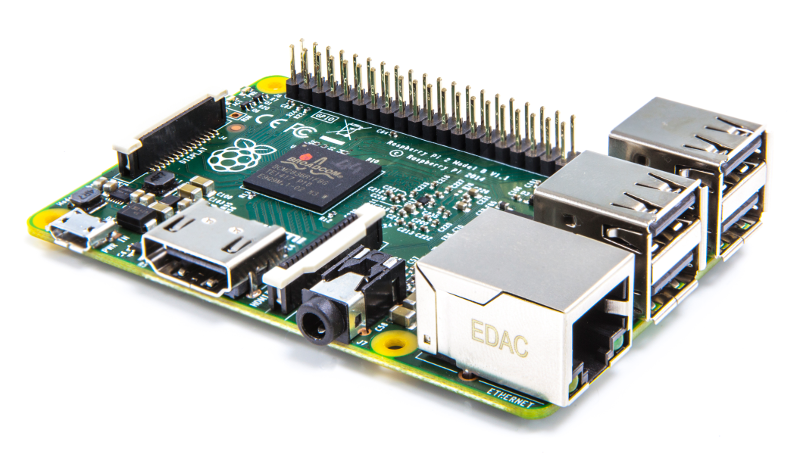
\includegraphics[width=5cm,natwidth=800,natheight=453]{rpi.png}
\end{figure}
\begin{itemize}
\item Petit ordinateur
\item Processeur ARM
\item 35 \$
\end{itemize}
\end{frame}

\begin{frame}
\frametitle{Dépendances des tâches}
\begin{figure}[center]
\includegraphics[width=12cm,natwidth=915,natheight=511]{GrapheSpe.png}
\end{figure}
\end{frame}

\begin{frame}
\frametitle{Objectifs (1/3)}
Noyau $\Rightarrow$ Système minimal
\begin{itemize}
\item UART
\item Interruptions
\item Horloge
\end{itemize}
\end{frame}

\begin{frame}
\frametitle{Objectifs (2/3)}
UART $\Rightarrow$ Système interactif
\begin{figure}[center]
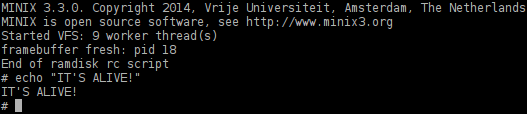
\includegraphics[width=12cm,natwidth=527,natheight=114]{console.png}
\end{figure}
\end{frame}

\begin{frame}
\frametitle{Objectifs (3/3)}
Périphériques $\Rightarrow$ Système utile
\begin{itemize}
\item Framebuffer
\item GPIO
\item I2C
\item ...
\end{itemize}
\end{frame}

\begin{frame}
\frametitle{Démonstration}
% \begin{figure}[center]
% 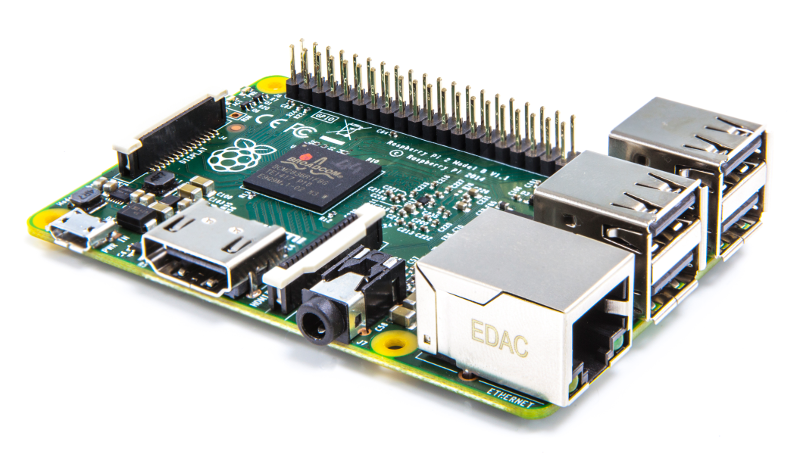
\includegraphics[width=5cm,natwidth=800,natheight=453]{rpi.png}
% \end{figure}
\end{frame}

\begin{frame}
\frametitle{État d'avancement}
Fait :
\begin{itemize}
\item Micro-noyau
\item UART
\item Framebuffer
\item GPIO
\end{itemize}

À faire :
\begin{itemize}
\item I2C
\item RTC
\item ...
\end{itemize}
\end{frame}

\begin{frame}
\frametitle{Conclusion}
% \begin{figure}[center]
% 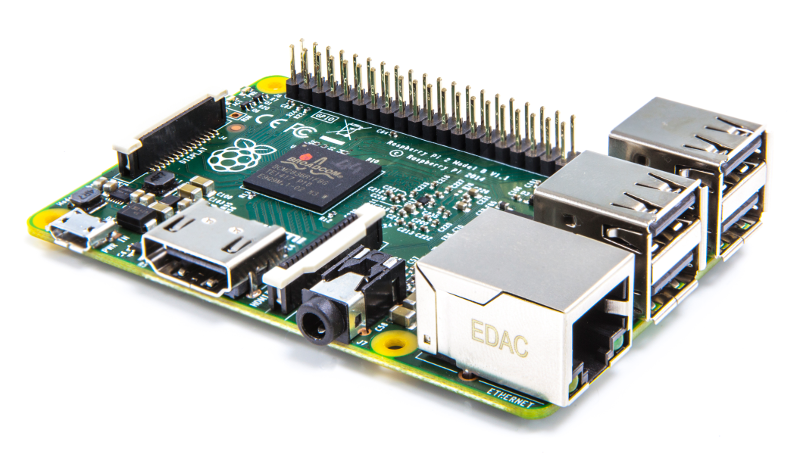
\includegraphics[width=5cm,natwidth=800,natheight=453]{rpi.png}
% \end{figure}
\end{frame}

\end{document}
